\subsection{Từ khoá continue, break, pass}
\label{keyloop}
Trong vòng lặp, ta cần chú ý ba từ khoá quan trọng là \texttt{continue}, \texttt{break} và \texttt{pass}.
\subsubsection{Continue}
Sử dụng từ khoá \texttt{continue} khi người lập trình muốn bỏ qua giá trị hiện tại, tiếp tục thực hiện vòng lặp với giá trị tiếp theo.\par
\begin{figure}[h]
	\centering
	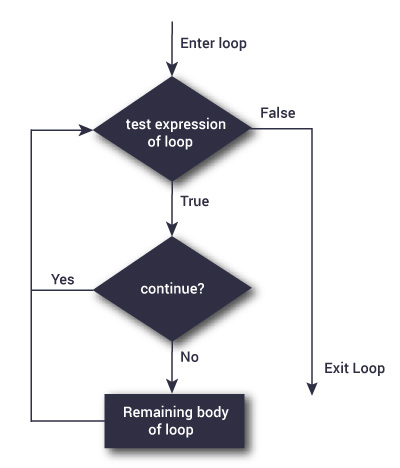
\includegraphics[width=0.4\linewidth]{img/continue}
	\caption{Mô tả cách thức hoạt động của từ khoá continue}
\end{figure}
\textbf{Ví dụ:} Tính căn bậc 2 của các phần tử trong dãy cho trước, bỏ qua các phần tử âm:\\
\rule{\linewidth}{0.2mm}\par
\begin{linenumbers}
	\texttt{\textcolor{red}{import} math}\par
	\smallskip
	\texttt{array = [1, 4, -5, 25, -8, 16]}\par
	\texttt{\textcolor{red}{for} i \textcolor{red}{in} array:}\par
	\qquad\texttt{\#skip element which is less than 0}\par
	\qquad\texttt{\textcolor{red}{if} i < 0:}\par
	\qquad\qquad\texttt{continue}\par
	\qquad\texttt{\textcolor{blue}{print}(math.sqrt(i))}\par
\end{linenumbers}
\rule{\linewidth}{0.2mm}\par
\noindent
\resetlinenumber
Kết quả cho ra ở Console:\\
\rule{\linewidth}{0.2mm}\par
\begin{linenumbers}
	\texttt{1.0}\par
	\texttt{2.0}\par
	\texttt{5.0}\par
	\texttt{4.0}\par
\end{linenumbers}
\rule{\linewidth}{0.2mm}\par
\resetlinenumber
\newpage
\subsubsection{Break}
Sử dụng từ khoá \texttt{break} khi người lập trình muốn dừng và thoát khỏi vòng lặp ngay lập tức.\par
\begin{figure}[h]
	\centering
	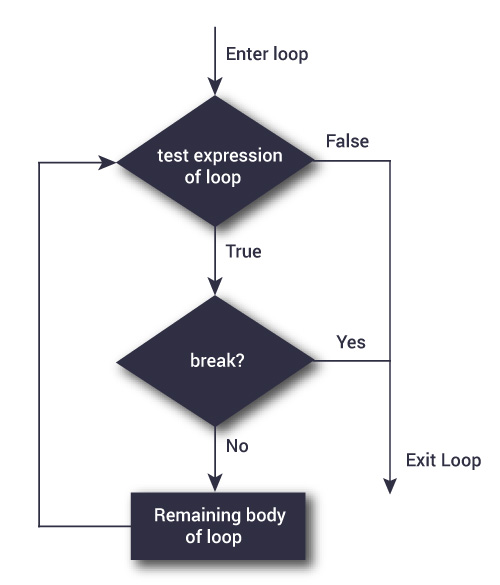
\includegraphics[width=0.4\linewidth]{img/break}
	\caption{Mô tả cách thức hoạt động của từ khoá break}
\end{figure}
\noindent
\textbf{Ví dụ:} Duyệt một chuỗi cho trước, lưu từng ký tự của chuỗi đó vào chuỗi mới, gặp kí tự 'E' thì ngừng lại:\\
\rule{\linewidth}{0.2mm}\par
\begin{linenumbers}
	\texttt{string = "contentE0xp"}\par
	\texttt{result = ""}\par
	\texttt{\textcolor{red}{for} i \textcolor{red}{in} string:}\par
	\qquad\texttt{\textcolor{red}{if} i == 'E':}\par
	\qquad\qquad\texttt{break}\par
	\qquad\texttt{result += i}\par
	\texttt{\textcolor{blue}{print}(result)}\par
\end{linenumbers}
\rule{\linewidth}{0.2mm}\par
\noindent
\resetlinenumber
Kết quả cho ra ở Console:\\
\rule{\linewidth}{0.2mm}\par
\begin{linenumbers}
	\texttt{content}\par
\end{linenumbers}
\rule{\linewidth}{0.2mm}\par
\resetlinenumber
\newpage
\subsubsection{Pass}
Khi người lập trình viết một vòng lặp hoặc một hàm, nhưng chưa có ý tưởng gì cho nó, thì có thể sử dụng từ khoá \texttt{pass} để thêm vào như là một câu lệnh giữ chỗ.\par
Nói một cách khác, \texttt{pass} là một lệnh trống, không làm gì cả. Python quy định các hàm và vòng lặp không được để trống. Vì thế, sử dụng từ khoá \texttt{pass} như là một câu lệnh để hợp thức hoá quy định trên.\par
Ví dụ về từ khoá \texttt{pass}:\\
\rule{\linewidth}{0.2mm}\par
\begin{linenumbers}
	\texttt{array = ['p', 'a', 's', 's']}\par
	\texttt{\textcolor{red}{for} i \textcolor{red}{in} array:}\par
	\qquad\texttt{pass}\par
	\texttt{\textcolor{blue}{print}("Pass successfully!")}\par
\end{linenumbers}
\rule{\linewidth}{0.2mm}\par
\noindent
\resetlinenumber
Kết quả cho ra ở Console:\\
\rule{\linewidth}{0.2mm}\par
\begin{linenumbers}
	\texttt{Pass successfully!}
\end{linenumbers}
\rule{\linewidth}{0.2mm}\par
\resetlinenumber
\newpage